\chapter{进一步工作}

\section{缺陷}

本文在此前的篇幅已经叙述过与 watchOS 、 LeapMotion 这些相关硬件开发上不可逾越的困难,在性能和功耗都严重受到限制 watchOS 上,交互消息的通信和处理都非常关键,一个良好的设计能够让各部分硬件顺利工作。然而软件是依赖硬件设计而成,因此接下来我们考虑在硬件实现本身和择备交互方案本身存在的问题。

\subsection{硬件缺陷}

作为一个原型项目,本文实现上使用 LeapMotion 完成对手部的的建模和识别,但 LeapMotion 自身却又限制在必须与一个桌面端系统进行连接,这就极大的限制了交互的范围和场景,不能在其他场景下使用。

在文\cite{Bailly:2012:SNP:2207676.2208576}中,Gilles 等人将一颗深度摄像头绑定在鞋子顶部,并在用户和腰部设置一个处理硬件用于识别交互,从而在鞋子顶部的上方制造了交互区域。类似的,我们可以设计图\ref{fig:hardware}所示的一个可移动的 LeapMotion 识别方案。

\begin{figure}[H]
    \centering
    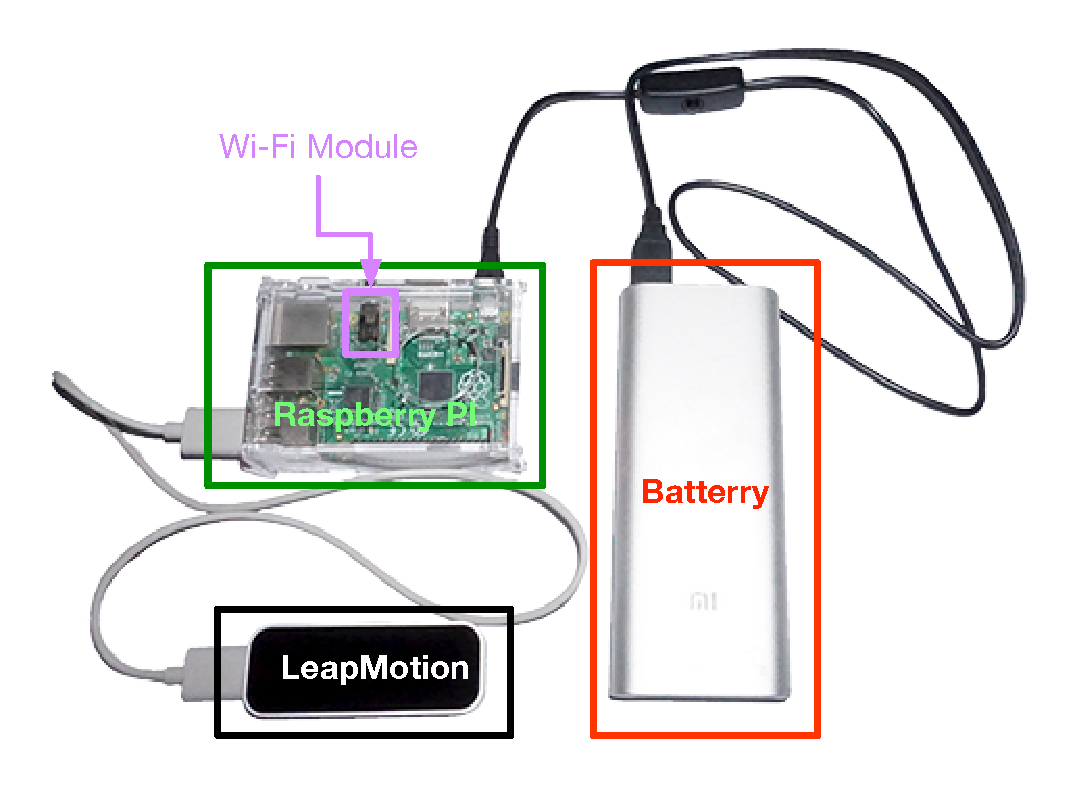
\includegraphics[width=0.6\textwidth]{figures/hardware}
    \caption{\kaishu \textbf{硬件结构}: 图中由三部分硬件分别为一个 5V-2A 输出功率的移动电源、一个组装了 WiFi 模组的树莓派 B+、一个 LeapMotion 硬件}
    \label{fig:hardware}
\end{figure}

在这个方案中,移动电源提供5V-2A 的输出功率,驱动树莓派;树莓派通过 WiFi 模组进而连接服务器进行交互信息通信,而 LeapMotion 则通过 USB 连接到树莓派上,只要树莓派上能够使用 LeapMotion 的软件部分,则此方案能够解决交互范围受限的问题。

遗憾的是,LeapMotion 软件要求宿主 OS 至少具备 2GB RAM,且 SDK 也仅能在 Ubuntu Linux 上得到支持,当前的树莓派第二代 B+仅有 512MB RAM,无法得到应用,但随着 Windows 10能够在树莓派第三代上运行,我们有望看到未来当树莓派扩展到2GB RAM 时能够搭载 Windows 平台将图 \ref{fig:hardware} 的方案得到应用。

\subsection{交互缺陷}

\section{改进方向}

\subsection{识别方式}

本文在手部信息的检测上使用了 LeapMotion 硬件作为解决问题的关键,但实际上 LeapMotion 是一项作为桌面端交互或虚拟现实交互的输入设备而产生的,这与

\subsection{交互感知中心}

在 \ref{sub:im-arch} 一节中,我们讨论了通信架构的设计,实际上这一设计也适用于一般情况。

\begin{figure}[H]
    \centering
    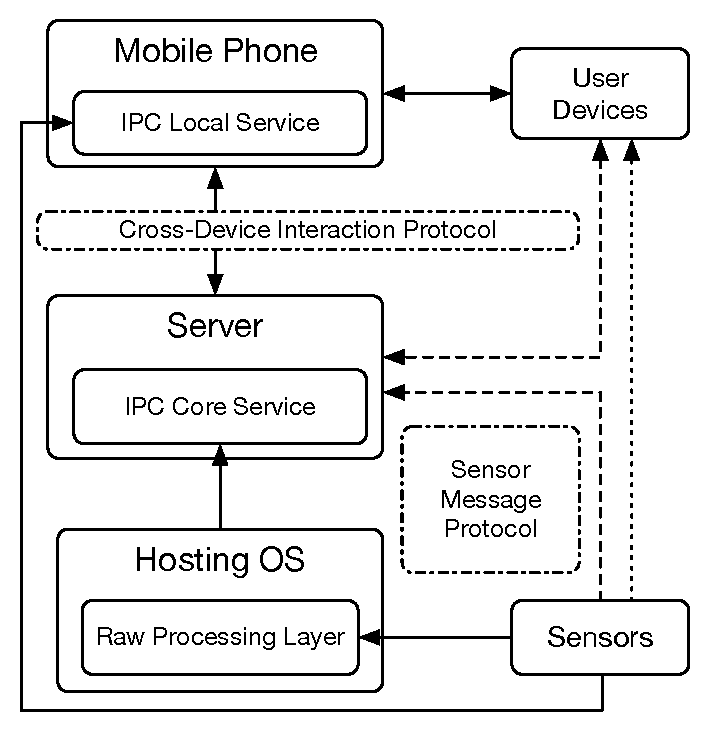
\includegraphics[width=0.4\textwidth]{figures/universe-arch}
    \caption{\kaishu \textbf{通用通信架构}: 交互感知中心(IPC)}
    \label{fig:universe-arch}
\end{figure}

图 \ref{fig:universe-arch} 展示了对通信架构设计的推广,并在服务端和客户端引入了交互感知中心(Interaction Perception Center, IPC 是一个基于桌面端和移动端设备的跨平台交互解决方案)服务\cite{Changkun:2015ipc}。不同的传感器先在与其连接的桌面端系统上按传感器各自的传感器处理协议(Sensor Handle Protocol, SH协议)对原始数据进行初步加工,再由 OS 将这些消息集中发送给服务端交给 IPC 核心服务进行处理进行二次加工,完成后再由服务端请求层按跨设备交互协议(Cross-Device Interaction Protocol, CDI协议)进行封装并分发给相应的设备;另一方面,当 IPC 核心服务不可用时,传感器的宿主 OS 依然能与客户端的本地 IPC 服务进行通信,使得在服务器离线状态下依然能够响应一些简单的交互。

当我们将 IPC 这一形式化人机交互模型引入,实现 IPC 核心服务的 SH 协议屏蔽掉了硬件之间的差异,而通过 CDI 协议方便的实现了用户设备与 IPC 服务之间的通信,通过 IPC 的数据的分析和加工,通过


\section{结束语}

本文对智能手表上现有的交互形式进行了备择设计,与主流交互不同,备择交互更像是编程语言上的一个语法糖,其侧重于临时、快捷、简便的实现一个用户期望的输入。在本次的设计中,我们克服了从硬件品台到软件框架上的种种缺陷,实现了一套非接触形式的点按、滑动、ForceTouch备择交互方案。同时,在克服这些缺陷中发展出来的各方面设计给与了我们很多的启示。

人机交互的创新往往伴随着硬件和软件的结合,在软件层的方法有时往往会受到硬件平台的各种限制,但这则是另一个更大的话题。
